\documentclass[12pt]{article}
\setlength\parindent{0pt}
\usepackage{amsmath}
\usepackage{lscape}
\usepackage{graphicx}
\usepackage{fullpage}
\usepackage[margin=0.8in]{geometry}
\setlength{\parskip}{4mm}
\def\LL{\left\langle}   % left angle bracket
\def\RR{\right\rangle}  % right angle bracket
\def\LP{\left(}         % left parenthesis
\def\RP{\right)}        % right parenthesis
\def\LB{\left\{}        % left curly bracket
\def\RB{\right\}}       % right curly bracket
\def\PAR#1#2{ {{\partial #1}\over{\partial #2}} }
\def\PARTWO#1#2{ {{\partial^2 #1}\over{\partial #2}^2} }
\def\PARTWOMIX#1#2#3{ {{\partial^2 #1}\over{\partial #2 \partial #3}} }
\newcommand{\BE}{\begin{displaymath}}
\newcommand{\EE}{\end{displaymath}}
\newcommand{\BNE}{\begin{equation}}
\newcommand{\ENE}{\end{equation}}
\newcommand{\BEA}{\begin{eqnarray}}
\newcommand{\EEA}{\nonumber\end{eqnarray}}
\newcommand{\EL}{\nonumber\\}
\newcommand{\la}[1]{\label{#1}}
\newcommand{\ie}{{\em i.e.\ }}
\newcommand{\eg}{{\em e.\,g.\ }}
\newcommand{\cf}{cf.\ }
\newcommand{\etc}{etc.\ }
\newcommand{\Tr}{{\rm tr}}
\newcommand{\etal}{{\it et al.}}
\newcommand{\OL}[1]{\overline{#1}\ } % overline
\newcommand{\OLL}[1]{\overline{\overline{#1}}\ } % double overline
\newcommand{\OON}{\frac{1}{N}} % "one over N"
\newcommand{\OOX}[1]{\frac{1}{#1}} % "one over X"
\pagenumbering{gobble}
\begin{document}
\Large
\centerline{\sc{Exercise -- Gravity and the Laws of Motion}}

\normalsize

In this exercise, you'll explore the laws of gravity and of motion. There isn't a homework assignment attached to this exercise, but you can expect to see questions like these on Exam 2 (a week from Tuesday).

Remember that these exercises are not meant for you to do alone; you should work with others near you on them, and should raise your hand and ask questions as you have them.

\section{The Law of Gravity}

Newton's law of gravity says that two objects whose masses are $m_1$ and $m_2$, and whose centers
are a distance $r$ apart, exert a force on each other of 

$$
F = \frac{Gm_1m_2}{r^2}.
$$

Here $G$ is a very small number that tells us how strong gravity is in our universe. We don't need to
know its value, since we will always just be interested in how the gravitational force {\it changes}.


Consider first only Earth and Mars. Earth is about nine times more massive than Mars.

\begin{center}
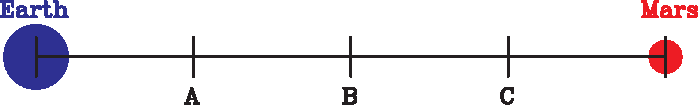
\includegraphics[width=0.5\textwidth]{earth-mars-crop.pdf}
\end{center}

 Two students, A and B, are debating the relative strengths of the forces on Earth and Mars.
	
	\begin{center}
		

	\begin{minipage}{0.9\textwidth}{\bf Student A:} It seems like Earth ought to exert a larger force on Mars than Mars exerts on Earth. Gravity depends on the mass of the planet creating the gravity, right? This is why the Earth has more gravity than the Moon. So since the more massive planet should create more gravity, Earth ought to pull on Mars with nine times more force than Mars pulls on Earth.
	
	\bigskip
	
	{\bf Student B:} Actually, shouldn't it go the other way around? Think about objects here on Earth. A big rock weighs more than a little rock because it has more mass. So the more massive planet ought to {\it feel} more gravity. This means that Mars pulls on Earth with nine times more force than Earth pulls on Mars!
	\end{minipage}
	\end{center}

\newpage

Which one is correct? If both of them are correct (or neither one is), explain how they are both correct (or incorrect), then explain whether Earth's gravitational force on Mars is larger than Mars' gravitational force on Earth.

\vspace{2in}

How do the arguments made by the two students above connect to the terms in the law of gravity, $F = \frac{Gm_1m_2}{r^2}$?

\vspace{1.5in}

Remember that Earth is nine times more massive than Mars. Is there a spot between Earth and Mars where a spacecraft would experience no gravitational force at all -- where Earth's gravity and Mars' gravity would counteract each other?

If so, where is that spot?

\begin{center}
	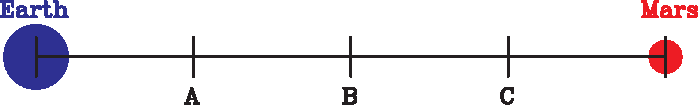
\includegraphics[width=0.5\textwidth]{earth-mars-crop.pdf}
\end{center}

\newpage

\section{The Law of Motion}

We've now figured out how gravity creates a force on objects. What do forces do?

The answer is given by Newton's law of motion:
	\begin{center}
	
	
	\begin{minipage}{0.9\textwidth}
		
		Forces cause objects to accelerate. The amount of acceleration is equal to the size of the force divided by the object's mass.
		
	\end{minipage}
\end{center}

Make sure you understand the difference between {\it force} and {\it acceleration} from gravity:

\begin{itemize}
\item {\bf Force} describes the weight of an object -- how hard gravity pulls on it.
\item {\bf Acceleration} describes its movement in response to that pull -- how fast it falls.
\end{itemize}


Consider the billiard ball and the feather in the evacuated tube: the billiard ball experienced more force than the feather (it is heavier), but it accelerated at the same rate.

\bigskip


Here are Earth and Mars again:

\begin{center}
	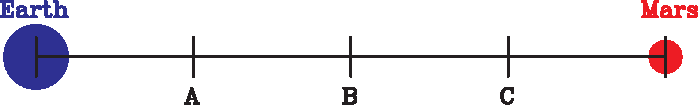
\includegraphics[width=0.5\textwidth]{earth-mars-crop.pdf}
\end{center}

Remember that Earth has nine times the mass of Mars. How does the {\it acceleration of Earth toward Mars} compare to the {\it acceleration of Mars toward Earth}?

\vspace{.7in}
	
	\newpage
	
An astronaut travels to the surface of the Moon, where there is no atmosphere. They drop a feather (mass 1 gram) and a stone (mass 1000 grams). Which one experiences {\it more gravitational force} from the Moon's gravity?

\vspace{2in}

Which one experiences {\it more acceleration due to gravity}? If your answer is different from the previous question, why is it different?

\vspace{2in}

The Solar System contains a lot of things besides the Earth and the Sun -- like the other planets! Do you think the gravity from those planets has any influence on Earth's orbit? If so, how big of an influence is it likely to have?

\newpage


	
\end{document}




